\newpage
\section{Grafica turtle}

Este o modalitate de desenare care se bazează pe câteva rutine simple. Ne putem imagina ca fiind un cursor care desenează 
linii drepte într-un plan cartezian. Cursorul are trei atribute: o locație, o orientare (sau o direcție) și un pix. 
Pixul are de asemenea, atribute: culoare, lățime și stare(desenare / inchis).\newline

Cursorul se muta cu comenzi care sunt relative la poziția sa, cum ar fi "înainte 10 pixeli" și "rotiți cu 90 de grade". 
Pixul purtat de cursor poate fi de asemenea controlat, având posibilitatea de a ii schimba culoarea sau lățimea.\newline

Un sistem complet de grafica necesita un flux de control, proceduri si recursivitate. Din aceste metode se pot construi forme mai complexe, cum ar fi pătrate, triunghiuri, cercuri și alte figuri compuse. 
Ideea de grafica turtle, de exemplu, este utilă într-un sistem Lindenmayer pentru generarea de fractali.\newline

Geometria graficii turtle funcționează oarecum diferit față de geometria carteziană, 
fiind bazată în primul rând pe noțiunea de vector (direcția relativă și distanța față de punctul de pornire).\newline

\subsection{Aplicare}

\lstset{language=C++}
\begin{lstlisting}
    class Turtle
    {
    public:
        Turtle(double x, double y, double dir);
        void rotate(double angle);
        void forward(double length, bool draw = true);
        Path getPath()const;
    private:
        double x,y,dir;
        Path path;
    };
\end{lstlisting}

De exemplu pentru a desena un triunghi echilateral cu lungimea laturilor de 100 de unitati.

\lstset{language=C++}
\begin{lstlisting}
    forward(100);
    rotate(PI/3);
    forward(100);
    rotate(PI/3);
    forward(100)
\end{lstlisting}

Fiecare comanda schimba starea Turtle-ului si a traseului desenat. 
Cele trei comenzi de forward desenează laturile triunghiului de lungime \(100\), adăugând latura la traseul total parcurs. 
Comenzile de rotate schimba direcția de desenare cu \(60\)\degree \footnote{in exemplul pentru desenare am folosit \(PI\) ca reprezentand \(180\)\degree, astfel \(180\degree \div 3 = 60\degree\)}. 
Dupa ultima comand de forward pixul se afla în punctul inițial de desenare, dar datorita lipsei unei comenzi rotate de \(60\)\degree, 
direcția de desenare este diferită de cea inițiala.\newline

Folosind structuri repetitive putem abstractiza metoda de desenare. De exemplu pentru desenarea unui poligon regulat convex:

\begin{lstlisting}
    polygon(nrOfEdges){
    for(i=1;i<nrOfEdges;i++):
        forward(2*PI/nrOfEdges);
        rotate(2*PI/nrOfEdges);	
    }
\end{lstlisting}

Pentru \verb|nrOfEdges=3| avem din nou un triunghi echilateral, pentru \verb|nrOfEdges=4| avem un pătrat, și asa mai departe. 
Folosind un \verb|nrOfEdges| destul de mare, lungimea laturii scade si  putem ajunge la o forma care într-un spațiu discret 
este similara cu un cerc.\newline 

\begin{figure}[H]
    \begin{center}
        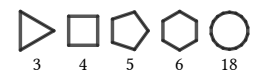
\includegraphics[scale=1]{imagini/turtle/circle.png}
        \caption{Desenarea unei forme similare cu un cerc}
        \label{fig:tabs}
    \end{center}    
\end{figure}

Extinzând aceste metode elementare de desenare putem ajunge la modalități de desenare pentru simboluri mai complexe 
formate din forme geometrice simple. (ex desenarea proiecției unui cilindru într-un plan 2D). \newline

\begin{figure}[H]
    \centering
    \subfloat[Joints]{{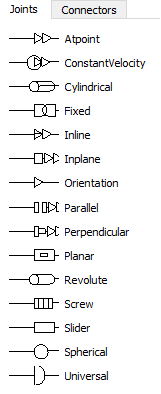
\includegraphics[scale=0.8]{imagini/turtle/joints.png} }}%
    \qquad
    \subfloat[Connectors]{{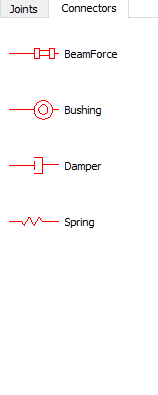
\includegraphics[scale=0.8]{imagini/turtle/connectors.png} }}%
    \caption{Simbolurile desenate prin turtle graphics pentru fiecare tip de connector sau joint}%
    \label{fig:example}%
\end{figure}


Pentru imeplementarea mea a acestui concept am adaugat funcțiile save() și load() pentru a eficientiza procesul de desenare.
Funcția save() salveaza starea curentă a clasei, și anume coordonatele x,y și direcția în acel moment. Astfel daca vrem să ne întoarcem 
într-un punct precedent nu mai este nevoie sa facem pașii necesari sa ne întoarcem in acel punct, ci putem apela direct functia load().\newline

Secventa de cod corespunzatoare implementării structurii de stare:

\lstset{language=C++}
\begin{lstlisting}
struct State
{
    State(double x, double y, double dir) 
    double m_x;
    double m_y;
    double m_dir;
};
\end{lstlisting}

Clasa adaptata:

\lstset{language=C++}
\begin{lstlisting}
class Turtle
{
public:
    Turtle(double x, double y, double dir);
    Turtle(QPointF start, double dir);
    void rotate(double angle);
    void forward(double length, bool draw = true);

    void save();
    void load();

    QPainterPath getPath()const;
private:
    QPainterPath m_path;
    State m_current;
    State m_saved;
};
\end{lstlisting}


